\chapter{Clase 5: Ejercicios de regresión lineal simple}

En esta clase se practican las herramientas estudiadas en las clases anteriores: diagrama de dispersión, correlación, recta de mínimos cuadrados, residuos, coeficiente de determinación y predicción. Se resuelve el ejercicio 3.1 del taller y se agregan los ejercicios 3.4 y 3.5. El 3.4 integra las dos rectas de regresión y las propiedades de las varianzas; el 3.5 permite estudiar una asociación negativa y estimar $X$ a partir de una respuesta observada.

\section{Ejercicio 3.1. Estrona en saliva y plasma}

Se realiza un estudio para establecer una ecuación mediante la cual se pueda utilizar la concentración de estrona en saliva ($X$) para predecir la concentración del esteroide en plasma libre ($Y$). Se extrajeron los siguientes datos de 14 varones sanos:

\begin{table}[H]
\centering
\small
\begin{tabular}{r|rr@{\qquad}r|rr}
Observación & $X$ & $Y$ & Observación & $X$ & $Y$ \\ \hline
1 & 1.4 & 30.0 & 8 & 14.0 & 49.0 \\
2 & 7.5 & 25.0 & 9 & 14.5 & 55.0 \\
3 & 8.5 & 31.5 & 10 & 16.0 & 48.5 \\
4 & 9.0 & 27.5 & 11 & 17.0 & 51.0 \\
5 & 9.0 & 39.5 & 12 & 18.0 & 64.5 \\
6 & 11.0 & 38.0 & 13 & 20.0 & 63.0 \\
7 & 13.0 & 43.0 & 14 & 23.0 & 68.0 \\
\end{tabular}
\caption{Concentraciones de estrona en saliva y plasma libre.}
\label{tab:clase5-estrona-datos}
\end{table}

Responda los siguientes incisos:
\begin{enumerate}
    \item[\textbf{a)}] Estudie la posible relación lineal entre ambas variables.
    \item[\textbf{b)}] Obtenga la ecuación que permite predecir la concentración en plasma a partir de la concentración en saliva.
    \item[\textbf{c)}] Determine cuánto varía la concentración en plasma por cada unidad adicional de estrona en saliva.
\end{enumerate}

\subsection*{Solución}
\begin{enumerate}
    \item[\textbf{a)}] El diagrama muestra una tendencia positiva aproximadamente lineal. La correlación cuantifica esta asociación:
    \[
    r=\frac{C_{XY}}{\sqrt{C_{XX}C_{YY}}}
    =\frac{957.775}{\sqrt{(423.3093)(2593.375)}}\approx0.9141.
    \]
    La asociación lineal de la muestra es marcada y positiva. El primer dato queda algo alejado de la recta, así que conviene revisar también la gráfica y no considerar el ajuste como exacto.
    \begin{figure}[H]
    \centering
    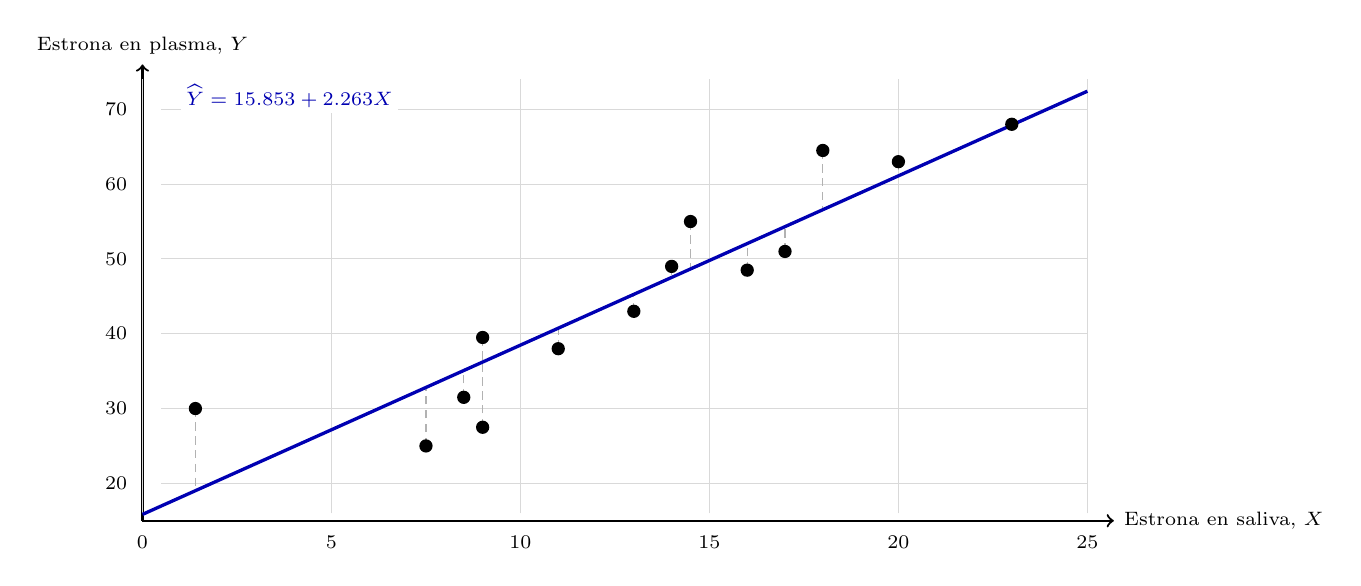
\begin{tikzpicture}[x=0.48cm,y=0.095cm,font=\scriptsize]
    \draw[->,thick] (0,15) -- (25.7,15) node[right] {Estrona en saliva, $X$};
    \draw[->,thick] (0,15) -- (0,76) node[above] {Estrona en plasma, $Y$};
    \foreach \xx in {0,5,10,15,20,25} {
        \draw[gray!30] (\xx,16) -- (\xx,74);
        \node[below=2pt] at (\xx,15) {\xx};
    }
    \foreach \yy in {20,30,40,50,60,70} {
        \draw[gray!30] (0.5,\yy) -- (25,\yy);
        \node[left=2pt] at (0,\yy) {\yy};
    }
    \foreach \x/\y/\yh in {
        1.4/30/19.02, 7.5/25/32.82, 8.5/31.5/35.08, 9/27.5/36.22,
        9/39.5/36.22, 11/38/40.74, 13/43/45.27, 14/49/47.53,
        14.5/55/48.66, 16/48.5/52.05, 17/51/54.32, 18/64.5/56.58,
        20/63/61.10, 23/68/67.89
    } {
        \draw[gray!60,densely dashed] (\x,\y) -- (\x,\yh);
    }
    \draw[blue!70!black,very thick] (0,15.85) -- (25,72.42);
    \foreach \x/\y in {
        1.4/30, 7.5/25, 8.5/31.5, 9/27.5, 9/39.5, 11/38, 13/43,
        14/49, 14.5/55, 16/48.5, 17/51, 18/64.5, 20/63, 23/68
    } {
        \fill[black] (\x,\y) circle (2.4pt);
    }
    \node[blue!70!black,fill=white,inner sep=2pt,anchor=west] at (1,71.8)
        {$\widehat Y=15.853+2.263X$};
\end{tikzpicture}
    \caption{Concentraciones de estrona, recta ajustada y residuos verticales.}
    \label{fig:clase5-estrona}
    \end{figure}

    \item[\textbf{b)}] Las sumas necesarias y las medias son
    \begin{align*}
    n&=14,& \sum x_i&=181.9,& \sum y_i&=633.5,\\
    \sum x_i^2&=2786.71,& \sum y_i^2&=31259.25,\\
    \sum x_iy_i&=9188.75.
    \end{align*}
    \[
    \bar x=\frac{181.9}{14}\approx12.9929,\qquad \bar y=\frac{633.5}{14}=45.25.
    \]
    Entonces,
    \begin{align*}
    C_{XX}&=2786.71-\frac{181.9^2}{14}\approx423.3093,\\
    C_{YY}&=31259.25-\frac{633.5^2}{14}=2593.375,\\
    C_{XY}&=9188.75-\frac{(181.9)(633.5)}{14}=957.775.
    \end{align*}
    Por mínimos cuadrados,
    \begin{align*}
    b_1&=\frac{C_{XY}}{C_{XX}}\approx2.2626,\\
    b_0&=\bar y-b_1\bar x\approx45.25-(2.2626)(12.9929)=15.8525.
    \end{align*}
    La ecuación estimada es
    \[
    \boxed{\widehat Y=15.8525+2.2626X.}
    \]
    Además, $R^2=r^2\approx0.8356$: la recta explica cerca del $83.56\%$ de la variación muestral de $Y$.

    \item[\textbf{c)}] La pendiente es $2.2626$. Según el ajuste, por cada unidad adicional de estrona en saliva, la concentración media estimada en plasma aumenta aproximadamente $2.26$ unidades. Esto describe una asociación, no demuestra causalidad.
\end{enumerate}

\section{Ejercicio 3.4. Comparación de dos métodos para medir nitrato}

Para estudiar la concentración de nitrato en el agua de un lago se comparan un método manual antiguo y un método automático. $X$ es la lectura manual y $Y$ la automática:

\begin{table}[H]
\centering
\small
\begin{tabular}{r|rr@{\qquad}r|rr}
Muestra & $X$ & $Y$ & Muestra & $X$ & $Y$ \\ \hline
1 & 25 & 30 & 6 & 300 & 350 \\
2 & 40 & 80 & 7 & 270 & 240 \\
3 & 120 & 150 & 8 & 400 & 320 \\
4 & 75 & 80 & 9 & 450 & 470 \\
5 & 150 & 200 & 10 & 575 & 583 \\
\end{tabular}
\caption{Lecturas de nitrato por los métodos manual y automático.}
\label{tab:clase5-metodos-datos}
\end{table}

Responda los siguientes incisos:
\begin{enumerate}
    \item[\textbf{a)}] Halle el coeficiente de determinación para las dos variables.
    \item[\textbf{b)}] Examine si es razonable usar un modelo lineal.
    \item[\textbf{c)}] Si el modelo es apropiado, obtenga la recta de $Y$ sobre $X$ y prediga la lectura automática cuando la manual es $100$.
    \item[\textbf{d)}] Calcule para cada muestra $\widehat X$, $\widehat Y$ y los residuos $X-\widehat X$, $Y-\widehat Y$.
    \item[\textbf{e)}] Compare las medias de $X$ con $\widehat X$ y de $Y$ con $\widehat Y$.
    \item[\textbf{f)}] Calcule las medias de ambos conjuntos de residuos. ¿Era esperable el resultado?
    \item[\textbf{g)}] Calcule las varianzas muestrales de $X$, $\widehat X$, $Y$, $\widehat Y$ y de ambos conjuntos de residuos.
    \item[\textbf{h)}] Compare $s_X^2$ con $s_{\widehat X}^2$ y $s_Y^2$ con $s_{\widehat Y}^2$.
    \item[\textbf{i)}] Relacione $s_X^2$ con $s_{X-\widehat X}^2$ y $s_Y^2$ con $s_{Y-\widehat Y}^2$.
    \item[\textbf{j)}] Explique por qué $r^2$ se denomina grado de bondad del ajuste lineal.
\end{enumerate}

\subsection*{Solución}
\begin{enumerate}
    \item[\textbf{a)}] Las sumas centradas son $C_{XX}=322372.5$, $C_{YY}=292988.1$ y $C_{XY}=300503.5$. Por tanto,
    \[
    r^2=\frac{C_{XY}^2}{C_{XX}C_{YY}}
    =\frac{300503.5^2}{(322372.5)(292988.1)}\approx0.9561.
    \]
    El valor es el mismo para la regresión de $X$ sobre $Y$, pues $r^2$ es simétrico en las dos variables.

    \item[\textbf{b)}] La nube presenta una tendencia creciente aproximadamente lineal. Para revisar los residuos se usa la recta de mínimos cuadrados que se calcula en el inciso c): $\widehat Y=26.11496+0.93216X$. El gráfico no muestra una curva sostenida, aunque la muestra 8 presenta una desviación apreciable. La recta es razonable como resumen inicial, con cautela por el tamaño pequeño de la muestra y ese residuo.
    \begin{figure}[H]
    \centering
    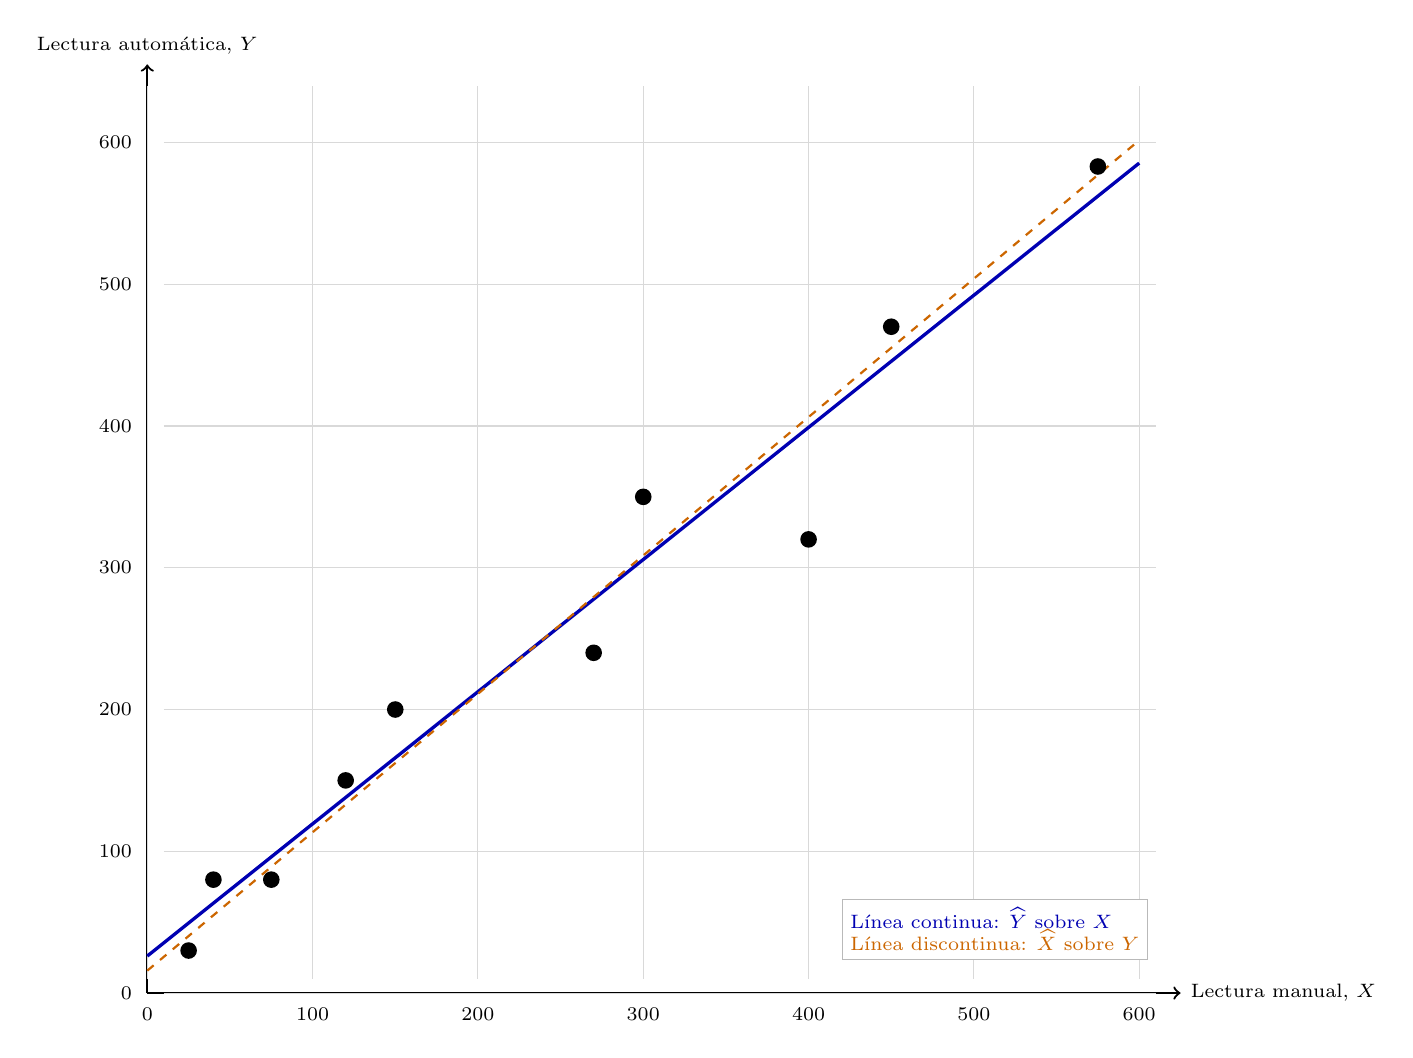
\begin{tikzpicture}[x=0.021cm,y=0.018cm,font=\scriptsize]
    \draw[->,thick] (0,0) -- (625,0) node[right] {Lectura manual, $X$};
    \draw[->,thick] (0,0) -- (0,655) node[above] {Lectura automática, $Y$};
    \foreach \xx in {0,100,200,300,400,500,600} {
        \draw[gray!30] (\xx,10) -- (\xx,640);
        \node[below=2pt] at (\xx,0) {\xx};
    }
    \foreach \yy in {0,100,200,300,400,500,600} {
        \draw[gray!30] (10,\yy) -- (610,\yy);
        \node[left=2pt] at (0,\yy) {\yy};
    }
    \draw[blue!70!black,very thick] (0,26.115) -- (600,585.412);
    \draw[orange!80!black,thick,dashed] (0,15.817) -- (600,601.5);
    \foreach \x/\y in {
        25/30,40/80,120/150,75/80,150/200,300/350,270/240,
        400/320,450/470,575/583
    } {
        \fill[black] (\x,\y) circle (3pt);
    }
    \node[draw=gray!55,fill=white,align=left,anchor=west,inner sep=3pt] at (420,45)
        {\textcolor{blue!70!black}{Línea continua: $\widehat Y$ sobre $X$}\\
         \textcolor{orange!80!black}{Línea discontinua: $\widehat X$ sobre $Y$}};
\end{tikzpicture}
    \caption{Datos y rectas de regresión. La línea discontinua corresponde a $X$ sobre $Y$, reescrita en los mismos ejes; ambas rectas pasan por $(\bar x,\bar y)$.}
    \label{fig:clase5-metodos-ajustes}
    \end{figure}
    \begin{figure}[H]
    \centering
    \begin{tikzpicture}[x=0.021cm,y=0.034cm,font=\scriptsize]
    \draw[->,thick] (0,-105) -- (625,-105) node[right] {Lectura manual, $X$};
    \draw[->,thick] (0,-105) -- (0,110) node[above] {Residuo $Y-\widehat Y$};
    \foreach \xx in {0,100,200,300,400,500,600} {
        \draw[gray!30] (\xx,-100) -- (\xx,100);
        \node[below=2pt] at (\xx,-105) {\xx};
    }
    \foreach \yy in {-100,-50,0,50,100} {
        \draw[gray!30] (10,\yy) -- (610,\yy);
        \node[left=2pt] at (0,\yy) {\yy};
    }
    \draw[red!70!black,dashed,thick] (0,0) -- (610,0);
    \foreach \x/\e in {
        25/-19.42,40/16.60,120/12.03,75/-16.03,150/34.06,
        300/44.24,270/-37.80,400/-78.98,450/24.41,575/20.89
    } {
        \fill[blue!70!black] (\x,\e) circle (2.8pt);
    }
    \node[below right,fill=white,inner sep=1pt] at (400,-78.98) {8};
\end{tikzpicture}
    \caption{Residuos de la regresión de la lectura automática sobre la manual. La muestra 8 tiene el residuo negativo de mayor magnitud.}
    \label{fig:clase5-metodos-residuos}
    \end{figure}

    \item[\textbf{c)}] Se tiene $n=10$, $\sum x_i=2405$, $\sum y_i=2503$, $\sum x_i^2=900775$, $\sum y_i^2=919489$ y $\sum x_iy_i=902475$. Las medias son $\bar x=240.5$ y $\bar y=250.3$. Así,
    \begin{align*}
    b_1&=\frac{C_{XY}}{C_{XX}}=\frac{300503.5}{322372.5}\approx0.93216,\\
    b_0&=\bar y-b_1\bar x=250.3-(0.93216)(240.5)\approx26.11496.
    \end{align*}
    La recta es $\widehat Y=26.11496+0.93216X$. Para $X=100$,
    \[
    \widehat Y=26.11496+0.93216(100)\approx119.33,
    \]
    es decir, cerca de $119$ unidades en la escala automática.

    \item[\textbf{d)}] La regresión de $X$ sobre $Y$ es $\widehat X=-16.22041+1.02565Y$. Para la primera muestra, $\widehat X_1\approx14.55$, $X_1-\widehat X_1\approx10.45$, $\widehat Y_1\approx49.42$ y $Y_1-\widehat Y_1\approx-19.42$. La tabla reúne los cálculos para todas las muestras:
    \begin{table}[H]
    \centering
    \scriptsize
    \setlength{\tabcolsep}{5pt}
    \renewcommand{\arraystretch}{1.08}
    \begin{tabular}{r r r r r r r}
    \hline
    $i$ & $X$ & $Y$ & $\widehat X$ & $X-\widehat X$ & $\widehat Y$ & $Y-\widehat Y$ \\
    \hline
    1 & 25 & 30 & 14.55 & 10.45 & 49.42 & -19.42 \\
    2 & 40 & 80 & 65.83 & -25.83 & 63.40 & 16.60 \\
    3 & 120 & 150 & 137.63 & -17.63 & 137.97 & 12.03 \\
    4 & 75 & 80 & 65.83 & 9.17 & 96.03 & -16.03 \\
    5 & 150 & 200 & 188.91 & -38.91 & 165.94 & 34.06 \\
    6 & 300 & 350 & 342.76 & -42.76 & 305.76 & 44.24 \\
    7 & 270 & 240 & 229.94 & 40.06 & 277.80 & -37.80 \\
    8 & 400 & 320 & 311.99 & 88.01 & 398.98 & -78.98 \\
    9 & 450 & 470 & 465.84 & -15.84 & 445.59 & 24.41 \\
    10 & 575 & 583 & 581.73 & -6.73 & 562.11 & 20.89 \\
    \hline
    \end{tabular}
    \caption{Predicciones y residuos de ambas regresiones.}
    \label{tab:clase5-metodos-predicciones}
    \end{table}

    \item[\textbf{e)}] Las dos rectas de mínimos cuadrados con intercepto pasan por el punto de medias:
    \[
    \overline{\widehat X}=\bar X=240.5,\qquad \overline{\widehat Y}=\bar Y=250.3.
    \]

    \item[\textbf{f)}] Por consiguiente, $\overline{X-\widehat X}=0$ y $\overline{Y-\widehat Y}=0$. Era esperable: en un ajuste por mínimos cuadrados con intercepto, la suma de los residuos es cero. Las diferencias pequeñas al sumar la tabla se deben al redondeo.

    \item[\textbf{g)}] Usando varianzas muestrales con denominador $n-1=9$,
    \begin{align*}
    s_X^2&=35819.17,& s_{\widehat X}^2&=34245.74,& s_{X-\widehat X}^2&=1573.42,\\
    s_Y^2&=32554.23,& s_{\widehat Y}^2&=31124.23,& s_{Y-\widehat Y}^2&=1430.01.
    \end{align*}

    \item[\textbf{h)}] Las razones de varianzas son
    \[
    \frac{s_{\widehat X}^2}{s_X^2}\approx\frac{34245.74}{35819.17}=0.9561,
    \qquad \frac{s_{\widehat Y}^2}{s_Y^2}\approx\frac{31124.23}{32554.23}=0.9561.
    \]
    En ambos casos la varianza ajustada representa cerca de $r^2=95.61\%$ de la varianza original.

    \item[\textbf{i)}] Los valores ajustados y los residuos son ortogonales; por eso,
    \[
    s_X^2=s_{\widehat X}^2+s_{X-\widehat X}^2,\qquad
    s_Y^2=s_{\widehat Y}^2+s_{Y-\widehat Y}^2.
    \]
    En efecto, $35819.17\approx34245.74+1573.42$ y $32554.23\approx31124.23+1430.01$. La fracción residual es $1-r^2\approx0.04393$, cerca del $4.39\%$.

    \item[\textbf{j)}] $r^2$ es la proporción de variación muestral representada por la recta; $1-r^2$ es la fracción que permanece en los residuos. Aquí el ajuste explica cerca del $95.61\%$ de la variación en cada regresión. Un valor alto no implica igualdad exacta entre las lecturas ni demuestra causalidad.
\end{enumerate}

\section{Ejercicio 3.5. Tiempo desde la diálisis y creatinina}

En pacientes tratados con Captopril tras la suspensión de la diálisis se midieron los días transcurridos ($X$) y la concentración de creatinina ($Y$, en mg/dl):

\begin{table}[H]
\centering
\begin{tabular}{r|rrrrrrr}
Días, $X$ & 1 & 5 & 10 & 15 & 20 & 25 & 35 \\
Creatinina, $Y$ & 5.7 & 5.2 & 4.8 & 4.5 & 4.2 & 4.0 & 3.8 \\
\end{tabular}
\caption{Días desde la diálisis y concentración de creatinina.}
\label{tab:clase5-creatinina-datos}
\end{table}

Responda los siguientes incisos:
\begin{enumerate}
    \item[\textbf{a)}] Halle la ecuación lineal que mejor describe la creatinina en función del tiempo, el grado de bondad del ajuste y la varianza residual.
    \item[\textbf{b)}] ¿En qué porcentaje la variación de la creatinina es explicada por el tiempo transcurrido desde la diálisis?
    \item[\textbf{c)}] Si un paciente presenta $4.1$ mg/dl de creatinina, estime cuánto tiempo ha transcurrido desde la suspensión de la diálisis.
\end{enumerate}

\subsection*{Solución}
\begin{enumerate}
    \item[\textbf{a)}] La nube muestra una tendencia descendente. Las sumas son
    \[
    n=7,\quad \sum x_i=111,\quad \sum y_i=32.2,\quad
    \sum x_i^2=2601,\quad \sum y_i^2=150.9,\quad \sum x_iy_i=464.2.
    \]
    De ellas, $\bar x=15.8571$, $\bar y=4.6$, $C_{XX}=840.8571$, $C_{YY}=2.78$ y $C_{XY}=-46.4$. Entonces,
    \begin{align*}
    b_1&=\frac{C_{XY}}{C_{XX}}\approx-0.05518,\\
    b_0&=\bar y-b_1\bar x\approx5.47503,
    \end{align*}
    y la recta es
    \[
    \boxed{\widehat Y=5.47503-0.05518X.}
    \]
    La suma de cuadrados residual es $SSE\approx0.21957$. Como medida descriptiva, $SSE/n\approx0.03137\,(\text{mg/dl})^2$; para estimar la varianza del error del modelo con $n-2$ grados de libertad,
    \[
    s_e^2=\frac{SSE}{n-2}=\frac{0.21957}{5}\approx0.04391\,(\text{mg/dl})^2.
    \]
    \begin{figure}[H]
    \centering
    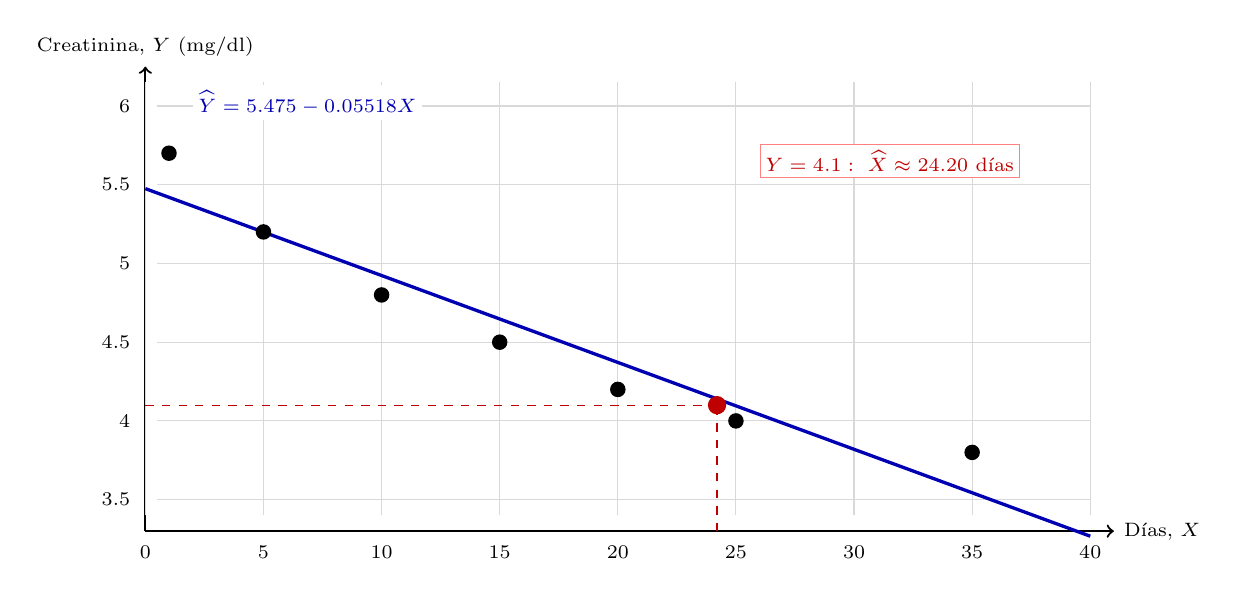
\begin{tikzpicture}[x=0.30cm,y=2cm,font=\scriptsize]
    \draw[->,thick] (0,3.3) -- (41,3.3) node[right] {Días, $X$};
    \draw[->,thick] (0,3.3) -- (0,6.25) node[above] {Creatinina, $Y$ (mg/dl)};
    \foreach \xx in {0,5,10,15,20,25,30,35,40} {
        \draw[gray!30] (\xx,3.4) -- (\xx,6.15);
        \node[below=2pt] at (\xx,3.3) {\xx};
    }
    \foreach \yy in {3.5,4,4.5,5,5.5,6} {
        \draw[gray!30] (0.5,\yy) -- (40,\yy);
        \node[left=2pt] at (0,\yy) {\yy};
    }
    \draw[blue!70!black,very thick] (0,5.475) -- (40,3.268);
    \foreach \x/\y in {1/5.7,5/5.2,10/4.8,15/4.5,20/4.2,25/4,35/3.8} {
        \fill[black] (\x,\y) circle (2.8pt);
    }
    \draw[red!75!black,dashed] (24.20,3.3) -- (24.20,4.1);
    \draw[red!75!black,dashed] (0,4.1) -- (24.20,4.1);
    \fill[red!75!black] (24.20,4.1) circle (3.3pt);
    \node[blue!70!black,fill=white,inner sep=2pt,anchor=west] at (2,6.02)
        {$\widehat Y=5.475-0.05518X$};
    \node[red!75!black,draw=red!50,fill=white,align=left,anchor=west,inner sep=2pt]
        at (26,5.65) {$Y=4.1:\ \widehat X\approx24.20$ días};
\end{tikzpicture}
    \caption{Creatinina según los días transcurridos, recta estimada y predicción inversa para $Y=4.1$.}
    \label{fig:clase5-creatinina}
    \end{figure}

    \item[\textbf{b)}] El coeficiente de determinación es
    \[
    R^2=r^2=\frac{C_{XY}^2}{C_{XX}C_{YY}}
    =\frac{(-46.4)^2}{(840.8571)(2.78)}\approx0.9210.
    \]
    El tiempo explica aproximadamente el $92.10\%$ de la variación muestral de la concentración de creatinina mediante el modelo lineal.

    \item[\textbf{c)}] Para estimar el tiempo $X$ a partir de $Y$, se ajusta la regresión de $X$ sobre $Y$; no se despeja $X$ de la ecuación de $Y$ sobre $X$. La pendiente es
    \[
    b_{X|Y}=\frac{C_{XY}}{C_{YY}}=\frac{-46.4}{2.78}\approx-16.69065,
    \]
    y el intercepto $a_{X|Y}=\bar x-b_{X|Y}\bar y\approx92.63412$. Por tanto,
    \[
    \widehat X=92.63412-16.69065Y.
    \]
    Para $Y=4.1$ mg/dl,
    \[
    \widehat X=92.63412-16.69065(4.1)\approx24.20\text{ días}.
    \]
    Como $4.1$ está dentro del intervalo de creatinina observado ($3.8$ a $5.7$ mg/dl), es una interpolación respecto del predictor $Y$. El tiempo estimado también queda dentro del rango observado de $1$ a $35$ días; en todo caso, es una estimación basada en una muestra pequeña.
\end{enumerate}

\clearpage